\chapter{大动态范围读出方案的设计与验证}
\label{ch:large_dynmaicrange}
一个探测器本征的探测性能由其构型和使用的探测介质材料决定。
探测器的本征分辨是相对固定的,在研制阶段,一般通过物理过程的蒙卡模拟(如Geant4)对其进行研究。
探测器实际的探测性能还取决于其读出设计,包括读出器件的选择、读出方案以及前端电子学的设计。
探测器的读出设计相对灵活,往往需要针对探测器的功能需求进行特殊设计,在研制阶段,一般经过多次的‘设计-实验验证’循环来确定最佳的设计方案。
合理的读出设计可以将探测器的本征探测性能发挥到极致,这也是探测器研制的主要目标。

对于PSD来说,它首先需要覆盖质子数$Z=1 \sim 20$的重离子探测。
根据第二章的描述(见\ref{sec:psd_principle}),相对论重离子在PSD塑闪单元条中的沉积能量近似正比于$Z^2$。因此,不同种类带电粒子在PSD中的输出信号幅度变化范围巨大,这对PSD探测单元模块读出方案的动态范围提出了上限要求。
另一方面,PSD同时需要对高能$\gamma$和高能$e$进行鉴别,即通过信号的有/无来判断入射粒子是否带电(见\ref{sec:psd_principle})。
为了降低$e/\gamma$误判率,PSD探测单元模块的读出方案需要足够敏感,能够有效区分带电粒子信号与电子学基线噪声信号,
这对其动态范围提出了下限要求。
一般的读出设计不能同时满足上述两方面的需求,我们需要对PSD探测单元模块的读出进行特殊设计,以满足其大动态范围的要求。

本章对PSD的读出方案设计进行了详细的论述,主要包括以下内容:PSD动态范围需求的估算,PSD读出方案的详细设计流程以及PSD大动态范围读出方案的实验验证。


\section{重离子在塑料闪烁体中的光产额}
\label{sec:dynamic_range:light_yield}
PSD使用PMT作为读出器件,P

\section{PSD动态范围需求的估算}
\label{sec:dynamic_range:estimation}

\section{大动态范围读出方案的设计}
\label{sec:dynamic_range:design}

\subsection{设计思路}
\label{sec:dynamic_range:readout_scheme}

\subsection{打拿极的选择}
\label{sec:dynamic_range:dynode_selection}

\begin{figure}[tb]
	\centering
	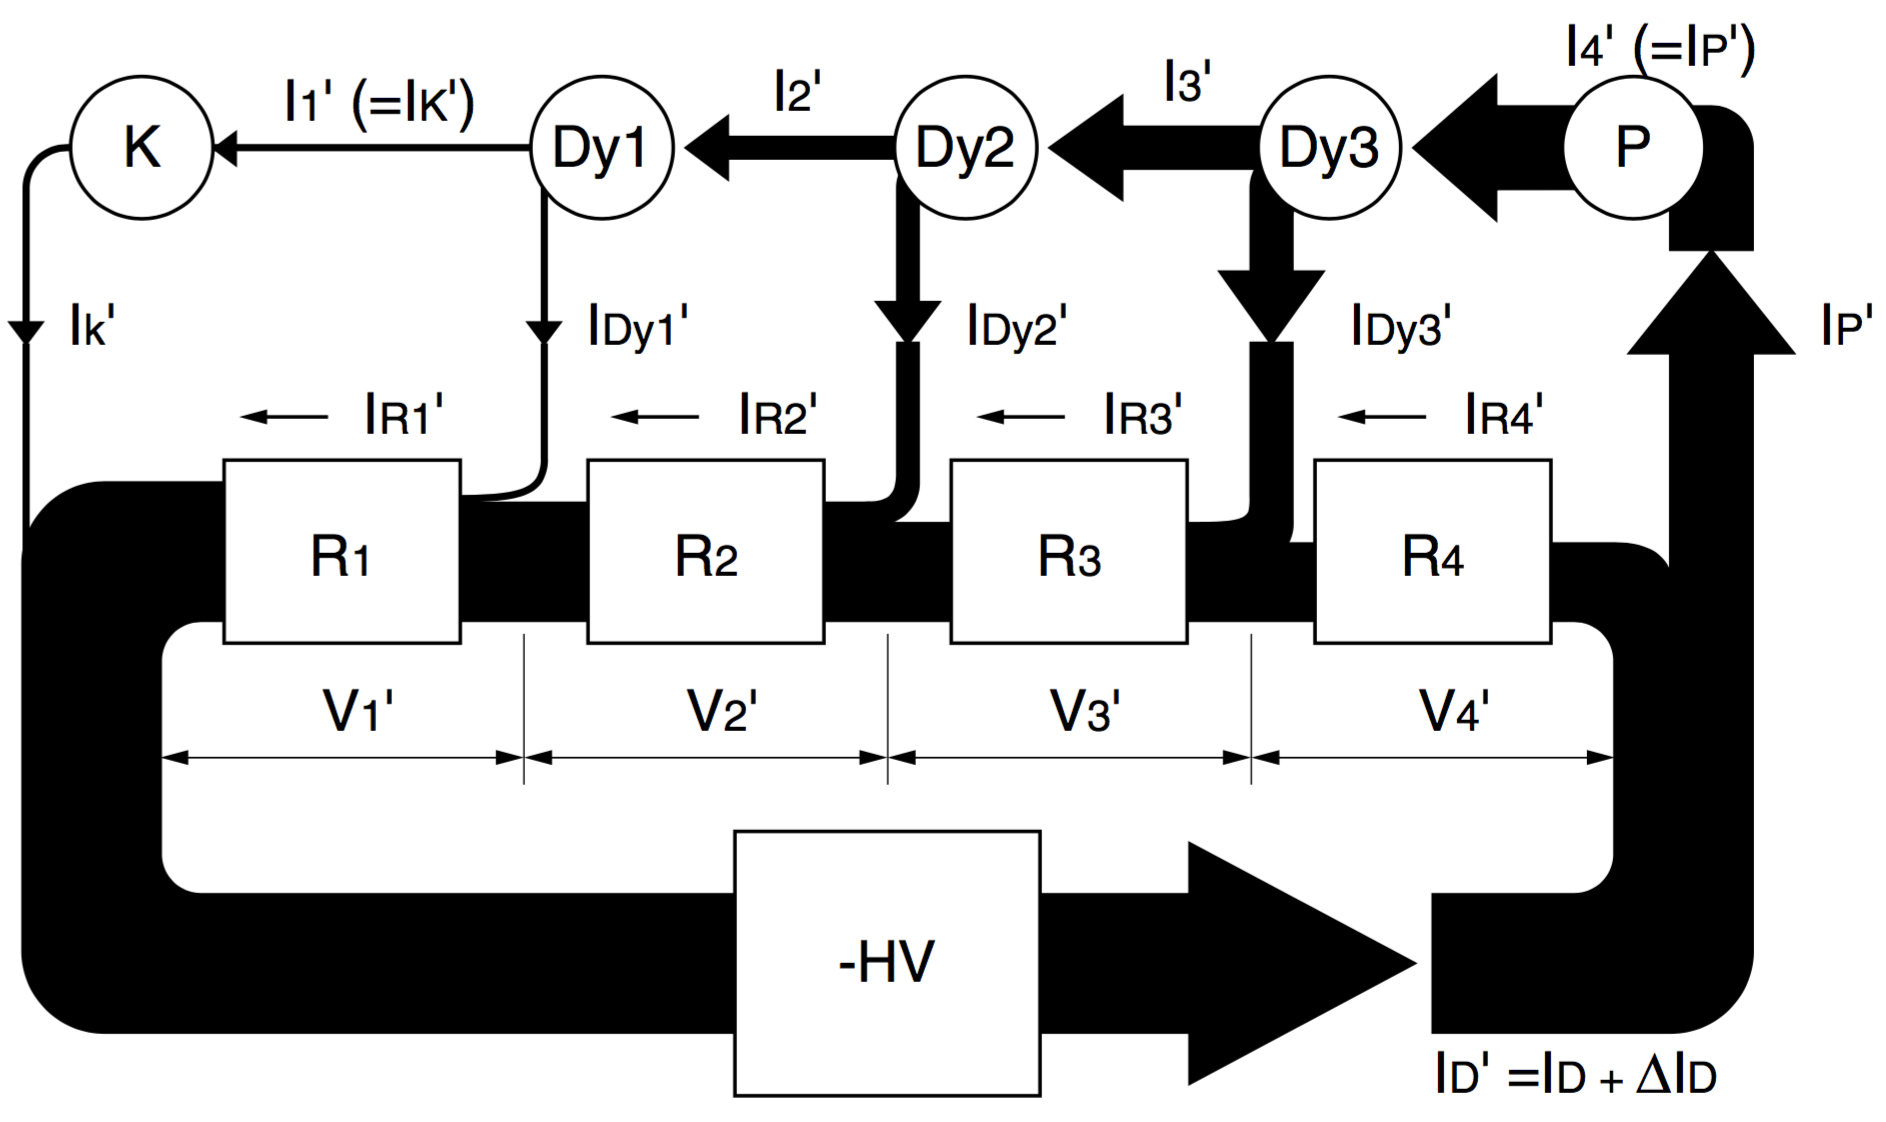
\includegraphics[width=0.9\textwidth]{chap/dynamic_range/fig/pmt_current_distribution_hamamatsu}
	\caption{Caption here}
	\label{fig:figure1}
\end{figure}

\subsection{分压器电路的设计}
\label{sec:dynamic_range:hv_divider}

\section{大动态范围读出方案的原理验证}
\label{sec:dynamic_range:verification}

\subsection{LED的测试}
\label{sec:dynamic_range:led}

\subsection{宇宙线的测试}
\label{sec:dynamic_range:cosmic_ray}

\subsection{中能轻核束流的测试}
\label{sec:dynamic_range:ion_beam}
